\documentclass{article}
\usepackage{graphicx} % Required for inserting images
\usepackage{amsmath,amssymb, amsthm}
\usepackage{algorithm}
\usepackage{algorithmic}
\usepackage{algpseudocode}

\usepackage{float}

\title{Mergeable Heaps}
\author{Kylind Reagan}
\date{September 2025}

\begin{document}

\maketitle

\section{Introduction}
A \textbf{mergeable heap} is a heap that supports the following operations:
\begin{enumerate}
    \item make\_heap() - Create \& return new heap with no elements.
    \item insert($H(x)$) - Insert node $x$ with key field already filled into heap $H$.
    \item  min($H$) - Return pointer to node in heap $H$ whose key is minimum
    \item extract\_min($H$) - Delete and return pointer to node with the minimum key in heap $H$.
    \item Union($H_1$, $H_2$) - Create and return new heap that contains all nodes from $H_1$ and $H_2$. $H_1, H_2$ destroyed in this operation.\\

    The mergeable heaps discussed below, \textbf{binomial heaps} and \textbf{fibonacci heaps} also support the following operations:\\
    \item Decrease\_key($H,x,k$)- Assign to node $x$ within heap $H$ new key with value k, assumed to be no greater than current key.
    \item Delete($H,x$): Delete node $x$ from heap $H$.
\end{enumerate}
If we do not need union, ordinary binary heaps are more useful in practical cases. However, union in binary heap is $\Theta(n)$!

\begin{table}[H]
    \centering
    \begin{tabular}{c|c|c|c}
    Procedure & Binary heap & Binomial heap & Fibonacci Heap \\
    & (Worst Case) & (Worst Case) & (amortized)\\
    \hline
    make\_heap & $\Theta(1)$ & $\Theta(1)$ & $\Theta(1)$\\
    insert & $\Theta(logn)$ & $O(logn)$ & $\Theta(1)$\\
    min & $\Theta(1)$ & $O(logn)$ & $\Theta(1)$\\
    extract\_min & $\Theta(logn)$ & $\Theta(logn)$ & $O(logn)$ \\
    union & $\Theta(n)$ & $\Theta(logn)$ & $\Theta(1)$\\
    decrease\_key & $\Theta(logn)$ & $\Theta(logn)$ & $\Theta(1)$\\
    delete & $\Theta(logn)$ & $\Theta(logn)$ & $\Theta(logn)$
    \end{tabular}
    \caption{Heap Comparison}
    \label{tab:placeholder}
\end{table}
\noindent All of them inefficient for search, thus delete and extract\_min suffer.
\section{Binomial Heaps}
\begin{figure}[htp]
    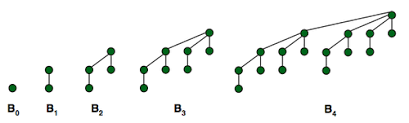
\includegraphics[width=\textwidth]{biheap.png}
    \caption{Binomial heaps $B_0$ to $B_4$}
    \label{tab:placeholder}
\end{figure}
\subsection{Introduction}
Binomial trees ($B_k$) are defined recursively as follows:\\
$B_0$ consists of a single node.\\
$B_k$, where $k = 1,...,n$ consist of 2 binomial trees $B_{k-1}$ linked together.\\
For binomial trees, the smaller root will be the leftmost child of the larger one.\\
\subsection{Properties of binomial trees}
Binomial trees have the following properties:
\begin{enumerate}
    \item There are $2^k$ nodes.
    \item The height of the tree is $k$.
    \item There are exactly \( \binom{k}{i}\) nodes at depth $i$ for $i=0,1,...,k$
    \item Root has degree $k$, which is greater than any other node.
    \begin{enumerate}
        \item Moreover, if children of root are numbered left to right by $k-1, k-2,...,0$ child $i$ is the root of subtree $B$.
    \end{enumerate}
\end{enumerate}
Corollary - Maximum degree of any node in an $n$-node binomial tree is $log(n)$.\\
Binomial heap $H$ is a set of binomial trees that satisfy the following:
\begin{enumerate}
    \item Each binomial tree in $H$ obeys min-heap property: key of a node is greater than or equal to the key of its parent (We say tree is min-heap-ordered).
    \item For any nonnegative integer $k$, there is at most 1 binomial tree $H$ whose root has degree $k$.
\end{enumerate}
The 1st property tells us the root contains the smallest key in the tree. The 2nd implies $n$-node binomial heap $H$ consists of at most $\lfloor lg(n)\rfloor + 1$ bits.\\
Roots of binomial trees in binomial heap organized in a linked list (called the root list).\\
\subsection{Operations in Binomial Heaps}
\subsubsection*{Binomial Link}
The \textsc{Binomial-Link} procedure makes one binomial tree the child of another, preserving the heap property. Specifically, it links two trees of the same degree by making the tree with the larger root key a child of the other. This guarantees that the resulting tree is still a binomial tree of higher degree.
\begin{algorithm}[H]
\caption{Binomial Link}
\begin{algorithmic}[1]
\PROCEDURE{Binomial-Link}{$(y, z)$}
    \COMMENT{Assumes $\text{key}[y] \geq \text{key}[z]$}
    \STATE $p[y] \GETS z$
    \STATE $\text{child}[y] \GETS \text{head}[z]$
    \STATE $\text{head}[z] \GETS y$
    \STATE $\text{degree}[z] \GETS \text{degree}[z] + 1$
\ENDPROCEDURE
\end{algorithmic}
\end{algorithm}
\subsubsection*{Merging Root Lists}
The \textsc{Merge} operation combines the root lists of two binomial heaps into a single linked list sorted by root degree. This step is purely structural and does not yet consolidate trees of the same degree.
\begin{algorithm}[H]
\caption{Merge Root Lists}
\begin{algorithmic}[1]
\PROCEDURE{Merge}{$(H_1, H_2)$}
    \COMMENT{Merge root lists of two binomial heaps}
    \STATE CREATE a new list $H$
    \STATE MERGE root lists of $H_1$ and $H_2$ into $H$ in order of increasing degree
    \RETURN $H$
\ENDPROCEDURE
\end{algorithmic}
\end{algorithm}
\subsubsection*{Union of Two Heaps}
The \textsc{Binomial-Heap-Union} operation first merges the root lists and then scans them to consolidate trees of the same degree, using \textsc{Binomial-Link}. The result is a valid binomial heap.
\begin{algorithm}[H]
\caption{Union}
\begin{algorithmic}[1]
\PROCEDURE{Binomial-Heap-Union}{$(H_1, H_2)$}
    \STATE $H \GETS$ \CALL{Merge}{$H_1,H_2$}
    \IF{$H = \emptyset$}
        \STATE \RETURN $H$
    \ENDIF
    \STATE LET $prev \GETS NIL$, $x \GETS \text{head}[H]$, $next \GETS \text{sibling}[x]$
    \WHILE{$next \neq NIL$}
        \IF{$\text{degree}[x] \neq \text{degree}[next]$ \OR 
            ($\text{sibling}[next] \neq NIL$ \AND $\text{degree}[next] = \text{degree}[\text{sibling}[next]]$)}
            \STATE $prev \GETS x$
            \STATE $x \GETS next$
        \ELSIF{$\text{key}[x] \leq \text{key}[next]$}
            \STATE $\text{sibling}[x] \GETS \text{sibling}[next]$
            \STATE \CALL{Binomial-Link}{$next, x$}
        \ELSE
            \IF{$prev = NIL$}
                \STATE $\text{head}[H] \GETS next$
            \ELSE
                \STATE $\text{sibling}[prev] \GETS next$
            \ENDIF
            \STATE \CALL{Binomial-Link}{$x, next$}
            \STATE $x \GETS next$
        \ENDIF
        \STATE $next \GETS \text{sibling}[x]$
    \ENDWHILE
    \STATE \RETURN $H$
\ENDPROCEDURE
\end{algorithmic}
\end{algorithm}

\subsubsection*{Insertion}
The \textsc{Insert} operation creates a new singleton binomial heap and unions it with the existing heap.


\begin{algorithm}[H]
\caption{Insert}
\begin{algorithmic}[1]
\PROCEDURE{Binomial-Heap-Insert}{$(H, x)$}
    \STATE CREATE a new heap $H'$ containing only node $x$
    \STATE $H \GETS$ \CALL{Binomial-Heap-Union}{$H, H'$}
\ENDPROCEDURE
\end{algorithmic}
\end{algorithm}

\subsubsection*{Extract Minimum}
The \textsc{Extract-Min} operation finds the root of minimum key, removes it, and reinserts its children (reversed into a valid root list). The result is a valid binomial heap with one fewer element.  


\begin{algorithm}[H]
\caption{Extract-Min}
\begin{algorithmic}[1]
\PROCEDURE{Binomial-Heap-Extract-Min}{$(H)$}
    \STATE FIND root $x$ in $H$ with minimum key
    \STATE REMOVE $x$ from root list of $H$
    \STATE LET $H'$ be a heap whose root list is the reverse of the list of $x$’s children
    \STATE $H \GETS$ \CALL{Binomial-Heap-Union}{$H, H'$}
    \STATE \RETURN $x$
\ENDPROCEDURE
\end{algorithmic}
\end{algorithm}

\section{Fibonacci Heaps}
\begin{figure}[htp]
    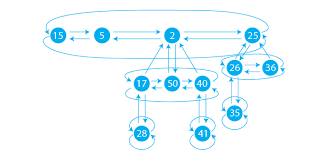
\includegraphics[width=\textwidth]{lesbianheap.png}
    \caption{Fibonacci heap}
    \label{tab:placeholder}
\end{figure}
\subsection{Introduction}
A Fibonacci heap is similar to Binomial heap, but it runs in $O(1)$ amortized time for any operations that do not involve delete. This makes it very desirable when delete and extract-min are used less frequently than other ops.\\
From a practical point of view, constant factors and programming complexities make them less desirable than binary/ k-nary heaps, making them more of a theoretical interest.\\
Fib heaps loosely based on binomial heaps, in fact, without decrease key and delete, each tree is like a binomial tree with a relaxed structure.\\
\subsection{Structure}
Trees in fib heap are min-heap-ordered and rooted, but unordered.\\
Children of $x$ are linked together in circular doubly linked list.\\
Each child $y$ has pointers to left and right siblings.\\
\\
Circular, doubly linked lists have 2 major advantages:
\begin{enumerate}
    \item Can remove a node from circular, doubly linked list in $O(1)$ time
    \item Given 2 structures, can concatenate (or "splice") into 1 circular, doubly linked list in $O(1)$ time.
\end{enumerate}
There are 2 other fields in each node:
\begin{enumerate}
    \item degree[$x$] = Number of children in child list of node $x$.
    \item mark[$x$] = boolean, whether $x$ has lost a child since the last time $x$ was made the child of another node
\end{enumerate}
Newly created nodes are unmarked (or false) and $x$ becomes unmarked whenever it is made a child of another node.\\
Given heap $H$ is accessed by pointer $min[H]$, the root of the tree containing the min key is called the \textbf{minimum node} of the fib heap. If $H$ empty, $min[H] = NIL$.\\
\subsection{Potential of Fib Heap}

For a given Fib Heap $H$, we indicate with $t(H)$ the number of trees in root list of H and by $m(H)$ the number of marked nodes in $H$. The potential of fib heap $H$ is then defined by...
\begin{align}
    \Phi = t(H) + 2m(H)
\end{align}

\subsection{Operations}
\subsubsection*{Make-Heap}
The \textsc{Make-Heap} operation creates and returns a new, empty Fibonacci heap.

\begin{algorithm}[H]
\caption{Make-Heap}
\begin{algorithmic}[1]
\PROCEDURE{Make-Heap}{}
    \STATE CREATE an empty heap $H$
    \RETURN $H$
\ENDPROCEDURE
\end{algorithmic}
\end{algorithm}

\subsubsection*{Insert}
The \textsc{Insert} operation adds a new node into the heap by inserting it into the root list.

\begin{algorithm}[H]
\caption{Insert}
\begin{algorithmic}[1]
\PROCEDURE{Fib-Heap-Insert}{$(H, x)$}
    \STATE $\text{degree}[x] \GETS 0$, $\text{parent}[x] \GETS NIL$, $\text{child}[x] \GETS NIL$
    \STATE $\text{mark}[x] \GETS FALSE$
    \STATE ADD $x$ to the root list of $H$
    \IF{$\text{min}[H] = NIL$ \OR $\text{key}[x] < \text{key}[\text{min}[H]]$}
        \STATE $\text{min}[H] \GETS x$
    \ENDIF
    \STATE $n[H] \GETS n[H] + 1$
\ENDPROCEDURE
\end{algorithmic}
\end{algorithm}

\subsubsection*{Minimum}
The \textsc{Minimum} operation returns the node containing the minimum key in the heap.

\begin{algorithm}[H]
\caption{Minimum}
\begin{algorithmic}[1]
\PROCEDURE{Fib-Heap-Minimum}{$(H)$}
    \RETURN $\text{min}[H]$
\ENDPROCEDURE
\end{algorithmic}
\end{algorithm}

\subsubsection*{Union}
The \textsc{Union} operation concatenates the root lists of two heaps and updates the minimum pointer.

\begin{algorithm}[H]
\caption{Union}
\begin{algorithmic}[1]
\PROCEDURE{Fib-Heap-Union}{$(H_1, H_2)$}
    \STATE CREATE a new heap $H$
    \STATE $\text{min}[H] \GETS \text{min}[H_1]$
    \STATE CONCATENATE root list of $H_2$ with root list of $H_1$
    \IF{$\text{min}[H_2] \neq NIL$ \AND (\text{min}[H] = NIL \OR $\text{key}[\text{min}[H_2]] < \text{key}[\text{min}[H]]$)}
        \STATE $\text{min}[H] \GETS \text{min}[H_2]$
    \ENDIF
    \STATE $n[H] \GETS n[H_1] + n[H_2]$
     \RETURN $H$
\ENDPROCEDURE
\end{algorithmic}
\end{algorithm}

\subsubsection*{Extract-Min}
The \textsc{Extract-Min} operation removes the node with the minimum key and restructures the heap.

\begin{algorithm}[H]
\caption{Extract-Min}
\begin{algorithmic}[1]
\PROCEDURE{Fib-Heap-Extract-Min}{$(H)$}
    \STATE $z \GETS \text{min}[H]$
    \IF{$z \neq NIL$}
        \FOR{each child $x$ of $z$}
            \STATE ADD $x$ to the root list of $H$
            \STATE $\text{parent}[x] \GETS NIL$
        \ENDFOR
        \STATE REMOVE $z$ from the root list of $H$
        \IF{$z = \text{sibling}[z]$}
            \STATE $\text{min}[H] \GETS NIL$
        \ELSE
            \STATE $\text{min}[H] \GETS \text{sibling}[z]$
            \STATE \CALL{Consolidate}{$H$}
        \ENDIF
        \STATE $n[H] \GETS n[H] - 1$
    \ENDIF
    \RETURN $z$
\ENDPROCEDURE
\end{algorithmic}
\end{algorithm}

\subsubsection*{Decrease-Key}
The \textsc{Decrease-Key} operation decreases the key of a given node, possibly cutting it from its parent and performing cascading cuts.

\begin{algorithm}[H]
\caption{Decrease-Key}
\begin{algorithmic}[1]
\PROCEDURE{Fib-Heap-Decrease-Key}{$(H, x, k)$}
    \IF{$k > \text{key}[x]$}
        \STATE ERROR: new key is greater than current key
    \ENDIF
    \STATE $\text{key}[x] \GETS k$
    \STATE $y \GETS \text{parent}[x]$
    \IF{$y \neq NIL$ \AND $\text{key}[x] < \text{key}[y]$}
        \STATE \CALL{Cut}{$H, x, y$}
        \STATE \CALL{Cascading-Cut}{$H, y$}
    \ENDIF
    \IF{$\text{key}[x] < \text{key}[\text{min}[H]]$}
        \STATE $\text{min}[H] \GETS x$
    \ENDIF
\ENDPROCEDURE
\end{algorithmic}
\end{algorithm}

\subsubsection*{Delete}
The \textsc{Delete} operation removes a node by first decreasing its key to $-\infty$ and then extracting the minimum.

\begin{algorithm}[H]
\caption{Delete}
\begin{algorithmic}[1]
\PROCEDURE{Fib-Heap-Delete}{$(H, x)$}
    \STATE \CALL{Fib-Heap-Decrease-Key}{$(H, x, -\infty)$}
    \STATE \CALL{Fib-Heap-Extract-Min}{$(H)$}
\ENDPROCEDURE
\end{algorithmic}
\end{algorithm}
\end{document}
